\documentclass[PICOReport.tex]{subfiles}

\begin{document}

{\bf Galactic Molecular Clouds} \\[0.3cm]
Stars form out of dense, gravitationally unstable subregions within molecular clouds. The efficiency of this conversion from molecular gas to stars is very low, as a result of the balance between turbulence, magnetic fields, feedback from young stars, and gravity over many scales in size and density \citep{McKee2007}.  Magnetic fields may play an important role in slowing the star formation process, by inhibiting motions of gas in the direction perpendicular to the field. However the degree to which 
magnetic fields reduce star formation efficiency is poorly constrained because of the difficulty of making detailed maps of magnetic fields over a large sample of molecular clouds.  With PICO we will answer the question of {\bf how do the magnetic fields that thread clouds inhibit the formation of dense, gravitationally unstable sub-structures within molecular clouds, and how does magnetic regulation affect the efficiency with which stars form?}

PICO will measure dust polarization over the entire sky, and since dust grains are known to align perpendicular to their local magnetic field \citep{Lazarian2007b,Andersson2015}, these observations will be used to create detailed maps of magnetic field morphology. With a best 1.1\arcmin~FWHM beam size PICO will be able to map all molecular clouds at better than \,1\,pc resolution out to 3.4\,kpc.  The BoloCam Galactic Plane Survey found 700 molecular clouds, recovering distances for approximately half their sample while covering roughly a third of the Galactic Plane \citep{EllsworthBowers2015}. PICO can therefore be expected to make highly detailed magnetic field maps of thousands of molecular clouds with thousands to hundreds of thousands of independent measurements per cloud, a huge improvement over the 10 nearby clouds mapped to the same level of detail with the {\em Planck} Satellite \cite{Planck:XXXV}.

Our goal is to use the PICO observations to measure:
\begin{itemize}
\item {\em The Balance between Gravity and Magnetic Support.} This is parameterized by the mass-to-flux ratio $\mu\,=\,M/M_{B}$, comparing M, the mass of a gas cloud to $M_{\Phi}\,=\,\Phi/2\pi G^{1/2}$, the maximum mass that can be supported by the magnetic flux ($\Phi$) through the cloud.
Where $\mu\,>\,1$\,the cloud cannot be supported by the magnetic field alone.
Current observations suggest that the envelopes of clouds can be supported against gravity by magnetic fields ($\mu\,<\,1$), but higher density structures such as cores and filaments are supercritical ($\mu\,>\,1$) and can thus collapse to form stars \citep{Crutcher2010}.  PICO will determine whether this model is true for all clouds and make detailed observations of the density scale magnetic flux is lost.
\item {\em The Balance between Turbulence and Magnetic Fields.} Turbulence also plays a crucial role in star formation. The turbulent gas motions will determine the initial range of gas density within the molecular cloud.  The balance between turbulent and magnetic fields, is characterized by the Alfv\'{e}n Mach number $\mathcal{M}_A\,=\,\sigma_k/v_A$, where $\sigma_k$ is the turbulent velocity width and $v_A\,=\,|B|/\sqrt{4\pi\rho}$ is the Alfv\'{e}n velocity.  If $\mathcal{M}_A\,<\,$1 then the magnetic field is strong enough to significantly influence gas motions. Recent Planck observations of ten nearby clouds have shown that low column density cloud structures statistically tend to align parallel to the magnetic field \cite{Planck:XXXII}, while high column density cloud structures have either no preferred alignment or in many cases align perpendicular to the magnetic field \citep{Planck:XXXV}.  These observations can only be reproduced in simulations if the large-scale magnetic field within molecular clouds is as strong or stronger than turbulence \citep{Soler2013,Chen2016,Mocz2018}.  PICO will determine whether the ``strong field'' case is true for molecular clouds of different ages and masses, and will measure the scale at which the cloud transitions from magnetic to turbulence and/or gravity dominated.
\end{itemize}

To measure these quantities we will apply established polarization analysis techniques:
\begin{itemize}
\item {\em Magnetic Field Dispersion:} Both \cite{Davis1951} and \cite{Chandrasekhar1953} showed that in the interstellar medium the dispersion in magnetic field direction angles can be used to estimate the magnetic field strength, if the turbulent velocity dispersion is known.  With PICO we will use the modern variations of this method \citep{Hildebrand2009,Houde2009,Houde2011} by fitting a model polarization angle dispersion power spectrum in order to constrain the projected magnetic field strength ($|B_{POS}|$), turbulent to magnetic field ratio ($\mathcal{M}_A$), and magnetized turbulence power spectrum .
\item {\em Polarization Modeling:} Measuring the statistical properties of the fraction of dust emission that is polarized and how this polarization level correlates with column density and magnetic field angle dispersion, can be used to constrain whether the field is strong or weak, where in the cloud is the magnetic field best traced, and how inclined the magnetic field is with respect to the plane of the sky \citep{Fissel2016, King2018}. 
\item {\em Comparing Polarization and Velocity Gradients:} Gradients in spectral line velocity for atomic and molecular gas have recently been shown to align perpendicular to the magnetic field \citep{GonzalezCasanova2017,Yuen2017, Lazarian2018}.  These gradients change from perpendicular to parallel to the magnetic field where the cloud becomes self-gravitating.  Most PICO target clouds have already been observed with Galactic plane molecular line surveys such as CHAMP, ThRUmms, MALT-90, and SEDGISM, so by comparing PICO maps the velocity structure we can determine where the energy balance between gravity and magnetic fields change.
\item {\em Cloud Structure Alignment the Magnetic Field:} {\em Planck} and BLASTPol observations have shown a statistically significant change in relative alignment of low (parallel) to high density (perpendicular) gas with respect to the magnetic field \citep{Planck:XXXV, Soler2017, Fissel2018}. As discussed above, this is consistent with cloud formation simulations where $\mathcal{M}_A\,\leq\,1$, or where the magnetic field is equal or stronger than the turbulent gas motions. The column density where the transition occurs seems to depend on both the degree of magnetization ($\mathcal{M}_A$), and formation history of the cloud \citep{Soler2017,Soler2017b}.
\end{itemize}
Each of the above analysis methods has different uncertainties and limitations.  However, by applying all four techniques to both PICO observations and synthetic polarization maps made from ``observing'' simulations of molecular clouds in models we will quantitatively compare theory and observations, strongly constraining both the magnetic field strength, Alfven Mach number, mass-to-flux ratio.  Once the magnetization parameters are determined by PICO, we can then compare the magnetization to the efficiency of star formation, measured from near and far-IR observations of protostars with {\em Herschel}, {\em Spitzer}, 
and {\em JWST}. 

{\bf PICO's ability to map thousands of clouds, is not possible with any other current or proposed polarimeter}. This large sample size is crucial, because dust polarization observations are sensitive to only the magnetic field projected on the plane of the sky.  Polarization maps, and therefore inferred magnetic field morphology will look very different for clouds of with different viewing angles, and also for young clouds versus clouds that have already formed stars that may provide radiative feedback.  {\bf Observing a large sample size of clouds will allow PICO to study the role of magnetic fields in star formation as a 
function age, mass, while accounting for statistically for different viewing angles.} \\

\begin{figure}
    \centering
    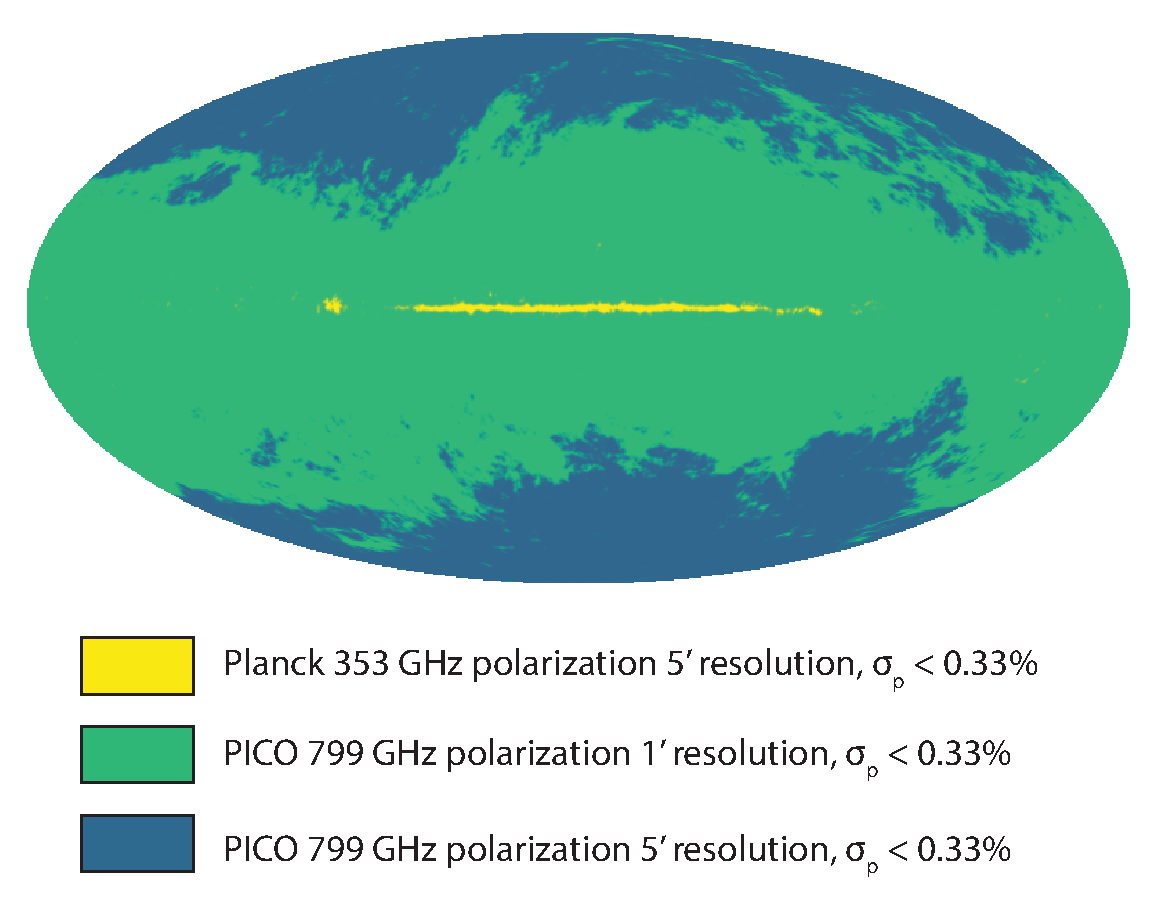
\includegraphics[width=4in]{images/Allsky_dust_fig.pdf}
    \caption{Caption}
    \label{fig:allsky}
  \end{figure}

{\bf Dust Physics - Grain Alignment} \\[0.3cm]
The association of interstellar polarization with elongated dust grains aligned by the interstellar magnetic field is well established \citep{Hall1949,Hiltner1949, Purcell1979,Spitzer1979}. For a review see \cite{Andersson2015}. Without a quantitative theory of grain alignment, it is impossible to properly model the magnetic field in the ISM using interstellar polarization observations. The last decade has been marked by significant advancements in developing the quantitative theory of grain alignment. In particular, the analytical model of grain alignment by radiative torques \citep{Lazarian2007a} has been developed with some of its predictions successfully confirmed \citep{Andersson2007,Andersson2010}. However, a number of key questions remain unanswered and this hinders the further progress of quantitative interpretation of the rich polarimetric data in relation to magnetic fields in the ISM. 

In particular, the efficiency of radiative torque alignment depends on whether the grains have enhanced magnetic susceptibility \citep{Lazarian2007b,Hoang2015}and whether the grain randomization is enhanced by magnetic turbulence \citep{Weingartner2008}. Observational testing of the theoretical predictions, in particular, at the extremes of low and high density lines of sight, can finally provide the community with comprehensive theory of grain alignment. PICO with its high sensitivity and resolution is ideally suited to make these key observations.

Very low density lines of sight through dust near very luminous stars can be used to explore the transition in RAT from alignment with respect to the radiation, to alignment with respect to the magnetic field. This transition depends strongly on the grain magnetic susceptibility.  PICO can explore grain alignment near hot stars with a strong UV continuum as well as cool stars, such as red giants and supergiants with much redder continua. These lines of sight will be very difficult to observe from balloon or airborne FIR and sub-mm polarimeters due to the low surface brightness and lack of all sky coverage.

At the other extreme, very high density lines of sight contain dust that is shielded from the interstellar radiation field, and show evidence for loss of grain alignment \citep{Goodman1995}(Jones et al. 2015). PICO will not be able to fully spatially resolve all of these dense, molecular cloud cores, but it will be able to measure fractional polarization and column depth for thousands of cores. The many contributing factors influencing measurements of grain alignment in dense cores, such as the local field direction (as determined by the surrounding position angles), level of turbulence (as seen in the surrounding polarimetry), direction and proximity to luminous infrared sources, presence of an embedded YSO (which may provide Mid-Infrared flux to align grains), and the type of embedded YSO (luminosity and SED) can be separated statistically with this large sample, an impossible task for ground based observations. These observations will provide a comprehensive assessment of grain alignment in dense molecular clouds. {\color{red} What measurements are necessary for this? Do we compare directions of polarization with magnetic fields measured in other ways? with radiation field directions? Are there critical complementary observations that we will assume/know we will have?} \\

{\bf Dust Physics - Composition} \\[0.3cm]
Spectroscopic features observed in both dust extinction and emission reveal the materials that compose interstellar dust. Strong extinction features at 9.7 and 18\,$\mu$m indicate much of the dust is in the form of amorphous silicates while features at 2175\,\AA, 3.3\,$\mu$m, and 3.4\,$\mu$m attest to abundant hydrocarbons. It is unknown, however, whether the silicate and carbonaceous materials coexist on the same grains (for instance, in a core-mantle structure) or whether they are segregated into distinct grain populations. If there are indeed multiple grain species, this will induce additional challenges for modeling the emission from interstellar dust in both total intensity and polarization at levels relevant for B-mode science \citep{Hensley2018}.

Polarimetry allows clear discrimination between these scenarios. Spectropolarimetry of dust extinction features have yielded a robust polarization signal in the 9.7\,$\mu$m silicate feature \citep[e.g.,][]{Smith2000}, indicating that the silicate grains are aligned with the interstellar magnetic field. In contrast, searches for polarization in the 3.4\,$\mu$m carbonaceous feature have yielded only upper limits, even along sightlines where silicate polarization is observed \citep{Chiar2006,Mason2007}. These data suggest that the silicate and carbonaceous materials cannot exist on the same grains. However, these studies are limited to only a few highly-extincted sightlines that may not typify the diffuse ISM.

Measuring polarized dust emission with PICO will provide a much more definitive test of these scenarios that extends to the most diffuse sightlines. If multiple dust species are contributing to the total dust emission, it is unlikely that they will all have identical SEDs, and therefore the fractional contribution of each grain type will vary with frequency. Likewise, it is unlikely that every grain type will have an identical intrinsic polarization fraction, and thus the total dust polarization fraction will vary with frequency. In constrast, the polarization fraction from compositionally homogeneous dust will be frequency-independent.

At odds with the spectropolarimetric evidence from dust extinction, current measurements of the polarization fraction of the dust emission with {\it Planck} \citep{Planck_Int_XXII} and BLASTPol \citep{Ashton2018} betray little to no frequency dependence across the full PICO frequency range (see Figure~). While some models with multiple dust species are ruled out by these data, many models still fall within the current uncertainties. In addition, the current data at $\nu > 353\,$GHz are from sightlines with much higher densities than the diffuse ISM, and thus may not be representative. 

In addition to silicon and carbon, dust grains are a reservoir for most of the interstellar iron, some of which may be in the form of superparamagnetic inclusions \citep{Draine2013}. The enhanced magnetic susceptibility from such inclusions results in the alignment from radiative torques becoming independent of the angle between the magnetic field and the radiation anisotropy \citep{Lazarian2007b,Hoang2015}, unlike for ordinary paramagnetic grains for which there is an explicit predicted dependence \citep{Lazarian2007a}. Thus, measuring grain alignment in the vicinity of bright stars with PICO, where the radiation direction is well-known, will provide a robust test for the presence of magnetic inclusions. Additionally, the emission from these inclusions will be polarized orthogonally to the electric dipole emission from the grain, leading to a decline in the polarization angle at low frequencies ($\nu \lesssim 100$\,GHz) and possibly a reversal in the polarization direction \citep{Draine2013}. Thus, PICO will also place direct constraints on the presence of magnetic inclusions through measurements of the dust polarization fraction.

In summary, PICO will dramatically improve the constraints on the properties of polarized dust emission and provide a definitive test of multi-component grain models, including the presence of magnetic inclusions. These insights will be directly inform modeling efforts in component separation

Meisner and Finkbeiner (2015) have determined a revised 2-component model for the diffuse Galactic thermal dust 
emission in the
far-infrared.
\begin{equation}
I_\nu \propto 8570\left(\frac{\nu}{GHz}\right)^{1.63} B_\nu(9.75 K) + 1.49 \left(\frac{\nu}{GHz}\right)^{2.82} B_\nu(15.7 K)
\end{equation}
Assuming an independent polarization for each of the components, a simple model for the polarization can be articulated.
\begin{equation}
p=\frac{p_1\times8570\left(\frac{\nu}{GHz}\right)^{1.63} B_\nu(9.75 K) + p_2\times1.49 \left(\frac{\nu}{GHz}\right)^{2.82} B_\nu(15.7 K)}{8570\left(\frac{\nu}{GHz}\right)^{1.63} B_\nu(9.75 K) + 1.49 \left(\frac{\nu}{GHz}\right)^{2.82} B_\nu(15.7 K)}
\end{equation}

Applying the noise estimates from PICO, 1000 simulations
were run for each combination of polarization values
for the two temperature components. Only frequency
channels 107 GHz and above are used, and the simulated
data are binned to the 7.9 arcminute beam of PICO?s
107 GHz channel. The uncertainties in each of the resulting
polarization fractions were estimated from the variance
of the simulation results. The resulting uncertainty of
the warmer component is expected to be 1.7\% and that
of the colder component is expected to be 1.3\%. \\

{\bf Diffuse Interstellar Medium} \\[0.3cm]
The diffuse ISM fills most of the volume of the Milky Way. It is a multi-phase medium, with magnetic fields, cosmic rays, and turbulence in rough energy equipartition \citep[e.g.,][]{Heiles:2005}. As the material that condenses to form molecular clouds, and eventually stars, and the material into which supernovae explode, the diffuse ISM is sculpted by a range of physics over many scales. Despite its importance, a comprehensive understanding of the diffuse ISM is challenging because of its diverse composition, its sheer expanse, and the multi-scale nature of the physics that shapes it. PICO is poised to revolutionize this field. With the unprecedented dynamic range summarized in Figure \ref{fig:allsky}, PICO will drastically expand our ability to study the diffuse ISM both as a function of environment and as a function of physical scale. Here we detail a few of the scientific areas where PICO will answer major open questions. \\

{\bf Diffuse Interstellar Medium - Structure Formation} \\[0.3cm]
Recent high-resolution observations of the diffuse ISM have revealed a wealth of complex structure, deeply influenced by the structure of the ambient magnetic field. The structure of the cold neutral medium (CNM) in particular is highly anisotropic, largely organized into filamentary structures that are aligned with the magnetic field \citep{Clark:2014}. Alignment between linear ISM structures and the magnetic field traced by dust polarization has recently been measured in both neutral hydrogen \citep{Clark:2015, Kalberla:2016} and dust emission \citep{Planck:XXXII}. The statistical properties of the density-magnetic field correlations can be described by cross-correlating the dust temperature ($T$) with the dust polarization field, decomposed into the rotationally invariant $E$- and $B$-modes. These measurements were made for the first time with \textit{Planck}, with several unexpected results. There is a positive $TE$ correlation in the diffuse ISM, as well as a nonunity ratio of $E$-mode to $B$-mode polarization ($EE/BB \sim 2$). These correlations are currently thought to be caused by the preferential elongation of density structures along the magnetic field \citep{Clark:2015, Planck:XXXVIII}. 
How do these quantities depend on scale and Galactic environment? The sensitivity and dynamic range of PICO will enable us to answer this question, which may in turn constrain properties of interstellar turbulence \citep[e.g.,][]{Caldwell:2017, Kandel:2017}. 


Perhaps even more surprisingly, the final \textit{Planck} data release reported a nonzero $TB$ correlation across a range of scales in the diffuse ISM \citep{Planck2018:XI}. Such a correlation implies that the density-polarization correlation is not parity invariant. PICO will make a much higher-fidelity measurement of the $TB$ correlation, and will either confirm or refute the \textit{Planck} detection. PICO will also constrain the $EB$ correlation value across the sky: $EB$ was found to be zero within \textit{Planck} uncertainty, but positive $TE$ and $TB$ correlations imply that at least a weak $EB$ correlation should exist. The origin of the $TB$ correlation is unknown. It has been speculated that the $TB$ correlation could be due to nonzero magnetic helicity, or some other parity-violating MHD property, or that the low-multipole $TB$ correlation may be related to the structure of the local large-scale magnetic field. PICO will test parity violation in the diffuse ISM, constrain models of magnetic helicity, and test models of the local Galactic magnetic field. {\color{red} Is this an opportunity for a figure showing how much better PICO will do for power spectra? Or maybe the cosmology sections have this covered}

Structure formation in the diffuse ISM is a key area of study motivating observations across the electromagnetic spectrum. PICO's observations will complement recently completed high dynamic range neutral hydrogen (\HI) surveys, such as \HI4PI \citep{HI4PI:2016} and GALFA-\hi \citep{Peek:2018}, as well as planned surveys of interstellar gas, most prominently with the Square Kilometer Array (SKA) and its pathfinders. One of the open questions in diffuse structure formation is how gas flows within and between phases of the ISM. A planned all-sky absorption line survey with SKA-1 will increase the number of measurements of the ISM gas temperature by several orders of magnitude \citep{McClure-Griffiths2015}. Quantitative comparisons of the ISM temperature distribution from SKA-1 and estimates of the magnetic field strength and coherence length scale from PICO will elucidate the role of the magnetic field in ISM phase transitions.


\end{document}

%\begin{figure}[!htb]
%\centering
%
\includegraphics[width=4cm]{images/example}
%\caption{example}
%\label{fig:im_3}
%\end{figure}
